\documentclass[12pt]{article}
\usepackage{amsmath}
\usepackage{graphicx}
\usepackage{hyperref}
\usepackage{listings}
\usepackage{color}
\usepackage{pythonhighlight}

\title{Operating System Course Report - First Half of the Semester}
\author{B class}
\date{\today}

\begin{document}

\maketitle
\newpage

\tableofcontents
\newpage

\section{Introduction}
This report summarizes the topics covered during the first half of the Operating System course. It includes theoretical concepts, practical implementations, and assignments. The course focuses on the fundamentals of operating systems, including system architecture, process management, CPU scheduling, and deadlock handling.

\section{Course Overview}
\subsection{Objectives}
The main objectives of this course are:
\begin{itemize}
    \item To understand the basic components and architecture of a computer system.
    \item To learn process management, scheduling, and inter-process communication.
    \item To explore file systems, input/output management, and virtualization.
    \item To study the prevention and handling of deadlocks in operating systems.
\end{itemize}

\subsection{Course Structure}
The course is divided into two halves. This report focuses on the first half, which covers:
\begin{itemize}
    \item Basic Concepts and Components of Computer Systems
    \item System Performance and Metrics
    \item System Architecture of Computer Systems
    \item Process Description and Control
    \item Scheduling Algorithms
    \item Process Creation and Termination
    \item Introduction to Threads
    \item File Systems
    \item Input and Output Management
    \item Deadlock Introduction and Prevention
    \item User Interface Management
    \item Virtualization in Operating Systems
\end{itemize}

\section{Topics Covered}

\subsection{Basic Concepts and Components of Computer Systems}
This section explains the fundamental components that make up a computer system, including the CPU, memory, storage, and input/output devices.

\subsection{System Performance and Metrics}
This section introduces various system performance metrics used to measure the efficiency of a computer system, including throughput, response time, and utilization.

\subsubsection{Matriks Performa}
\label{subsec:performance_matrix}

\quad Evaluasi performa sistem komputer merupakan salah satu aspek paling penting dalam menentukan efisiensi eksekusi program dan operasi sistem secara keseluruhan. Matriks performa menyediakan pengukuran yang dapat diandalkan untuk mengevaluasi efisiensi suatu sistem dalam mengeksekusi instruksi, mengelola proses, dan memaksimalkan sumber daya perangkat keras.\\

Beberapa komponen utama dari matriks performa termasuk \textit{Cycles Per Instruction (CPI)}, \textit{Clock Speed}, \textit{Latency}, \textit{Throughput}, \textit{Clock Rate}, dan \textit{Execution Time}. Berikut adalah penjelasan dari masing-masing komponen:\\

\textbf{1. Cycles Per Instruction (CPI):} Mengukur rata-rata jumlah siklus \textit{clock} yang diperlukan oleh prosesor untuk menyelesaikan satu instruksi. Rumusnya adalah:\\

\begin{equation}
CPI = \frac{\text{Total Siklus Clock}}{\text{Total Instruksi}}
\end{equation}\\

Semakin rendah \textit{CPI}, semakin efisien prosesor. \textit{CPI} dapat dioptimalkan dengan memperbaiki arsitektur seperti \textit{pipelining}, \textit{superscalar}, atau \textit{branch prediction}.\\

\textbf{2. Clock Speed:} Merupakan jumlah siklus \textit{clock} yang diselesaikan oleh prosesor dalam satu detik, diukur dalam \textit{Gigahertz (GHz)}. Meskipun \textit{clock speed} yang lebih tinggi biasanya menunjukkan kecepatan yang lebih baik, efisiensi arsitektur tetap memainkan peran penting.\\

\textbf{3. Latency:} Mengacu pada penundaan yang terjadi antara saat instruksi diberikan kepada prosesor dan saat instruksi mulai diproses. \textit{Latency} bisa berasal dari berbagai sumber, seperti memori, jaringan, atau disk.\\

\textbf{4. Throughput:} Jumlah pekerjaan atau instruksi yang dapat diselesaikan oleh sistem dalam satu satuan waktu. \textit{Throughput} yang lebih tinggi menunjukkan kemampuan sistem untuk memproses lebih banyak data atau instruksi dalam waktu yang lebih singkat.\\

\textbf{5. Clock Rate:} Didefinisikan sebagai jumlah siklus \textit{clock} per detik. Hubungannya dengan waktu eksekusi adalah:\\

\begin{equation}
\text{Clock Rate} = \frac{1}{\text{Waktu per Siklus Clock}}
\end{equation}\\

\textbf{6. Execution Time:} Waktu total yang dibutuhkan oleh sistem untuk menyelesaikan eksekusi suatu program. Rumusnya adalah:\\

\begin{equation}
\text{Execution Time} = \frac{\text{Jumlah Instruksi} \times \text{CPI}}{\text{Clock Rate}}
\end{equation}\\

\textbf{Interaksi Matriks Performa:} Matriks performa ini saling mempengaruhi satu sama lain. Sebagai contoh, \textit{clock speed} yang lebih tinggi dengan \textit{CPI} yang rendah akan meningkatkan \textit{throughput}, tetapi juga dapat meningkatkan konsumsi daya dan panas.\\

\textbf{Contoh Perhitungan:} Misalkan sebuah sistem memiliki \textit{clock rate} 2.5 GHz, \textit{CPI} 1.2, dan program membutuhkan 20 juta instruksi. Waktu eksekusi dihitung sebagai berikut:\\

\[
\text{Execution Time} = \frac{20 \times 10^6 \times 1.2}{2.5 \times 10^9} = 0.0096 \text{ detik}
\]\\

Sistem ini akan mengeksekusi program tersebut dalam 0.0096 detik.\\

\subsection{System Architecture of Computer Systems}
Describes the architecture of modern computer systems, focusing on the interaction between hardware and the operating system.

\subsection{Process Description and Control}
Processes are a central concept in operating systems. This section covers:
\begin{itemize}
    \item Process states and state transitions
    \item Process control block (PCB)
    \item Context switching
\end{itemize}

\subsection{Scheduling Algorithms}
This section covers:
\begin{itemize}
    \item First-Come, First-Served (FCFS)
    \item Shortest Job Next (SJN)
    \item Round Robin (RR)
\end{itemize}
It explains how these algorithms are used to allocate CPU time to processes.

\subsection{Process Creation and Termination}
Details how processes are created and terminated by the operating system, including:
\begin{itemize}
    \item Process spawning
    \item Process termination conditions
\end{itemize}

\subsection{Introduction to Threads}
This section introduces the concept of threads and their relation to processes, covering:
\begin{itemize}
    \item Single-threaded vs. multi-threaded processes
    \item Benefits of multithreading
\end{itemize}

\begin{figure}[h]
    \centering
    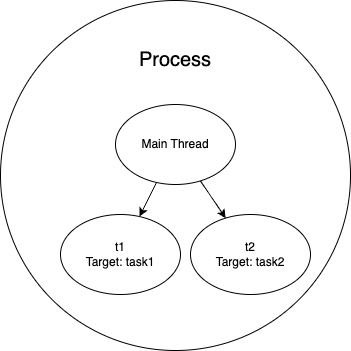
\includegraphics[width=0.5\textwidth]{/Users/khawaritzmi/Unhas/os_report_mid2024/b_class/asset/example.png}  % Sesuaikan nama file dan ukurannya
    \caption{Ini adalah gambar contoh dari multithreading.}
    \label{fig:contoh_gambar}
\end{figure}

Seperti yang terlihat pada Gambar \ref{fig:contoh_gambar}, inilah cara menambahkan gambar dengan keterangan.

\subsection{File Systems}
File systems provide a way for the operating system to store, retrieve, and manage data. This section explains:
\begin{itemize}
    \item File system structure
    \item File access methods
    \item Directory management
\end{itemize}

\subsection{Input and Output Management}
Input and output management is key for handling the interaction between the system and external devices. This section includes:
\begin{itemize}
    \item Device drivers
    \item I/O scheduling
\end{itemize}

\subsection{Deadlock Introduction and Prevention}
Explores the concept of deadlocks and methods for preventing them:
\begin{itemize}
    \item Deadlock conditions
    \item Deadlock prevention techniques
\end{itemize}

\subsection{User Interface Management}
This section discusses the role of the operating system in managing the user interface. Topics covered include:
\begin{itemize}
    \item Graphical User Interface (GUI)
    \item Command-Line Interface (CLI)
    \item Interaction between the user and the operating system
\end{itemize}

\subsection{Virtualization in Operating Systems}
Virtualization allows multiple operating systems to run concurrently on a single physical machine. This section explores:
\begin{itemize}
    \item Concept of virtualization
    \item Hypervisors and their types
    \item Benefits of virtualization in modern computing
\end{itemize}

\section{Assignments and Practical Work}
\subsection{Assignment 1: Process Scheduling}
Students were tasked with implementing various process scheduling algorithms (e.g., FCFS, SJN, and RR) and comparing their performance under different conditions.
\subsubsection{Group 1}
\begin{python}
    class Process:
    def __init__(self, pid, arrival_time, burst_time):
        self.pid = pid
        self.arrival_time = arrival_time
        self.burst_time = burst_time
        self.completion_time = 0
        self.turnaround_time = 0
        self.waiting_time = 0
\end{python}

\begin{table}[htbp] % Optional: For floating position
    \centering
    \begin{tabular}{|c|c|c|} % Defines number of columns and alignment (c = center, l = left, r = right). '|' creates vertical lines.
    \hline
    Header 1 & Header 2 & Header 3 \\ % Column headers
    \hline
    Row 1, Column 1 & Row 1, Column 2 & Row 1, Column 3 \\ % First row of data
    \hline
    Row 2, Column 1 & Row 2, Column 2 & Row 2, Column 3 \\ % Second row of data
    \hline
    \end{tabular}
    \caption{Your table caption} % Optional: For adding a caption
    \label{tab:your_label} % Optional: For cross-referencing the table
\end{table}

\subsection{Assignment 2: Deadlock Handling}
In this assignment, students were asked to simulate different deadlock scenarios and explore various prevention methods.

\subsection{Assignment 3: Multithreading and Amdahl's Law}
This assignment involved designing a multithreading scenario to solve a computationally intensive problem. Students then applied **Amdahl's Law** to calculate the theoretical speedup of the program as the number of threads increased.

\subsection{Assignment 4: Simple Command-Line Interface (CLI) for User Interface Management}
Students were tasked with creating a simple **CLI** for user interface management. The CLI should support basic commands such as file manipulation (creating, listing, and deleting files), process management, and system status reporting.

\subsubsection{Assignment 4: Simple Command-Line Interface (CLI) for User Interface Management}

\textbf{Soal:}

Buatlah sebuah program Command-Line Interface (CLI) sederhana yang mendukung operasi berikut:
\begin{itemize}
    \item Menampilkan daftar file di direktori saat ini.
    \item Membuat file baru.
    \item Menghapus file yang ada.
    \item Menampilkan bantuan (help) yang mencantumkan daftar perintah yang didukung oleh CLI.
\end{itemize}

\textbf{Petunjuk}:
\begin{itemize}
    \item Gunakan modul Python \texttt{os} untuk menangani operasi file dan direktori.
    \item Implementasikan perintah-perintah berikut:
        \begin{itemize}
            \item \texttt{list} untuk menampilkan file di direktori saat ini.
            \item \texttt{create <filename>} untuk membuat file baru dengan nama yang diberikan.
            \item \texttt{delete <filename>} untuk menghapus file dengan nama yang diberikan.
            \item \texttt{help} untuk menampilkan daftar perintah yang tersedia.
            \item \texttt{exit} untuk keluar dari CLI.
        \end{itemize}
\end{itemize}

\textbf{Jawaban:}

Berikut adalah implementasi Python untuk Command-Line Interface (CLI) sederhana tersebut:

\begin{python}
import os

def list_files():
    """Menampilkan daftar file di direktori saat ini."""
    files = os.listdir('.')
    if files:
        print("Daftar file di direktori saat ini:")
        for file in files:
            print(file)
    else:
        print("Direktori kosong.")

def create_file(filename):
    """Membuat file baru."""
    if os.path.exists(filename):
        print(f"File '{filename}' sudah ada.")
    else:
        with open(filename, 'w') as f:
            f.write("")  # Membuat file kosong
        print(f"File '{filename}' berhasil dibuat.")

def delete_file(filename):
    """Menghapus file."""
    if os.path.exists(filename):
        os.remove(filename)
        print(f"File '{filename}' berhasil dihapus.")
    else:
        print(f"File '{filename}' tidak ditemukan.")

def display_help():
    """Menampilkan daftar perintah yang tersedia."""
    print("Daftar perintah yang didukung:")
    print("1. list                - Menampilkan daftar file di direktori saat ini.")
    print("2. create <filename>    - Membuat file baru.")
    print("3. delete <filename>    - Menghapus file.")
    print("4. help                - Menampilkan bantuan.")
    print("5. exit                - Keluar dari CLI.")

def cli():
    """Fungsi utama untuk menjalankan Command-Line Interface (CLI)."""
    print("Selamat datang di Simple CLI!")
    display_help()
    
    while True:
        command = input(">>> ").strip().split()
        if not command:
            continue
        
        if command[0] == "list":
            list_files()
        elif command[0] == "create" and len(command) > 1:
            create_file(command[1])
        elif command[0] == "delete" and len(command) > 1:
            delete_file(command[1])
        elif command[0] == "help":
            display_help()
        elif command[0] == "exit":
            print("Keluar dari CLI.")
            break
        else:
            print("Perintah tidak valid. Ketik 'help' untuk bantuan.")

# Menjalankan CLI
if __name__ == "__main__":
    cli()
\end{python}

Program di atas akan menyediakan fungsi dasar CLI yang bisa melakukan beberapa operasi manajemen file, seperti menampilkan daftar file, membuat file, menghapus file, menampilkan bantuan, dan keluar dari CLI. Program ini juga menggunakan modul Python \texttt{os} untuk menangani operasi yang berhubungan dengan file dan direktori.

\subsection{Assignment 5: File System Access}
In this assignment, students implemented file system access routines, including:
\begin{itemize}
    \item File creation and deletion
    \item Reading from and writing to files
    \item Navigating directories and managing file permissions
\end{itemize}

\section{Conclusion}
The first half of the course introduced core operating system concepts, including process management, scheduling, multithreading, and file system access. These topics provided a foundation for more advanced topics to be covered in the second half of the course.

\end{document}